\chapter{Background on Computational Neurocience}
\label{sec:back}

The goal of this section is not to give a detailed description of most important concepts regarding computational neuroscience, but to give a brief overview of most basic and relevant concepts in the context of this work.

Due to the fact that there exist a large number of neuron models of all levels of complexity we present some basic and widely used single neuron models. They are of relevance to our work since they have been previously used in the study of the degeneracy problem.

Since our work concerns the study of the degeneracy problem in an oversimplified neuron network, we also describe how biophysical realistic neuron networks are built connecting different neurons. We describe synaptic dynamical models: electrical and chemical synapses, as well as, some mathematical models for neuron networks.

Some concepts are illustrated considering an example of a realistic biophysical network model of the basal ganglia, \cite{Rubin2004}, a part of the brain. The network models includes four neural structures: the thalamus (TC), the subthalamic nucleus (STN), the external segment of the globus pallidus (GPe) and the internal segment of the globus pallidus (GPi). We shall refer to this models as the \textit{STN-GPe-GPi-TC} model. During this research experience, I have also had the opportunity of working with this computational model. The goal was to understand how pathological rhythms in pakinsonian subjects, \cite{Gillies2017}, are originated.

The contents of this section are mainly based on \cite{Volume2009,book1,Abbott1996,Herz2006,Lourens2013}.

\section{Single neuron models}
The original Hodgkin-Huxley model for the generation of an action potential is presented. In addition, we introduce a more general class of models known as conductance-based models, which are based on the Hodgkin-Huxley formalism. Finally, we present some reduced and two-variable models which are of interest to perform a detailed mathematical analysis.

An exhaustive description of models is not presented. Moreover, models are presented from the mathematical perspective and less attention is given to biophysical interpretations. However, we believe that this section can help the reader to acquire the fundamental knowledge in computational neuroscience in order to contextualize our work.


\subsection{The Hodgkin-Huxley model}
The classic Hodgkin-Huxley model, \cite{Hodgkin1990}, suggests that an electrical circuit can represent electrical membrane activity. As a single-compartment model, neuron's spatial structure is neglected and the membrane potential of a neuron is described by a single variable $V$.

The model focus on the interplay of different ionic currents to generate spiking activity. It consist of four differential equations. One of them is for the membrane potential ($V$) and the remaining three equations for channel gating variables ($n$, $m$ and $h$) which represent the voltage-dependent channel kinetics. The channel opening and closing rates determine the current carried through the channel. Equations can be written as

\begin{equation}
    C\frac{dV}{dt} = - \bar{g}_{K}n^{4}(V-E_{K}) - \bar{g}_{Na}m^{3}h(V-E_{Na}) - \bar{g}_{L}(V-E_{L})
\end{equation}
\begin{equation}
    \frac{dn}{dt} = \frac{n_{\infty}(V)-n}{\tau_{n}(V)}
\end{equation}
\begin{equation}
    \frac{dm}{dt} = \frac{m_{\infty}(V)-m}{\tau_{m}(V)}
\end{equation}
\begin{equation}
    \frac{dh}{dt} = \frac{h_{\infty}(V)-h}{\tau_{h}(V)}
\end{equation}

where $C$ is the membrane capacitance, $\bar{g}_{K}$, $\bar{g}_{Na}$ and $\bar{g}_{L}$ are the potassium, sodium and leak maximal conductances and $E_{K}$, $E_{Na}$ and $E_{L}$ are the potassium, sodium and leak reversal potentials.

Ionic currents 

\begin{equation}
    I_{K} = \bar{g}_{K}n^{4}(V-E_{K}) \hspace{0.5cm} \text{and} \hspace{0.5cm} I_{Na} = \bar{g}_{Na}m^{3}h(V-E_{Na})
\end{equation}

are responsible for the generation of the action potential. However, the leak current

\begin{equation}
    I_{L} = \bar{g}_{L}(V-E_{L})
\end{equation}

represents all time-independent contributions to the membrane currents.

Fig. (\ref{photo1}) shows steady-states activation and inactivation functions ($n_{\infty}(V)$, $m_{\infty}(V)$ and $h_{\infty}(V)$) and time constants ($\tau_{n}(V)$, $\tau_{m}(V)$ and $\tau_{h}(V)$) on the Hodgkin-Huxley type model.

\begin{figure}[h]
  \begin{minipage}{0.5\linewidth}
  \begin{center}
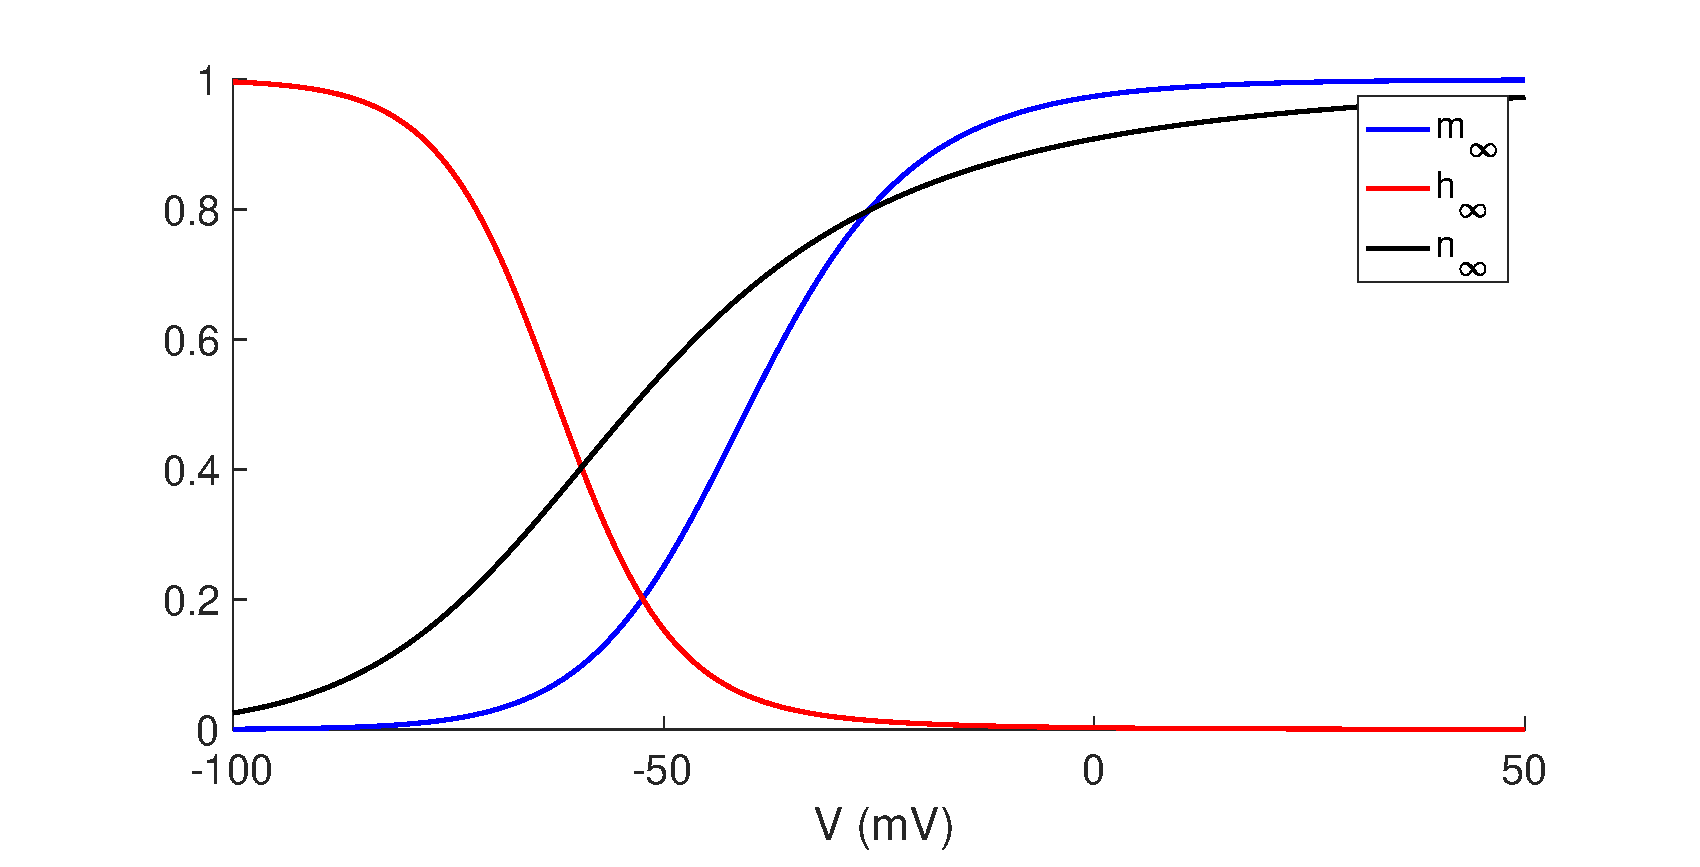
\includegraphics[width=1\linewidth]{Images/photo1_1.eps}
\end{center}
  \end{minipage} 
  \begin{minipage}{0.5\linewidth}
  \begin{center}
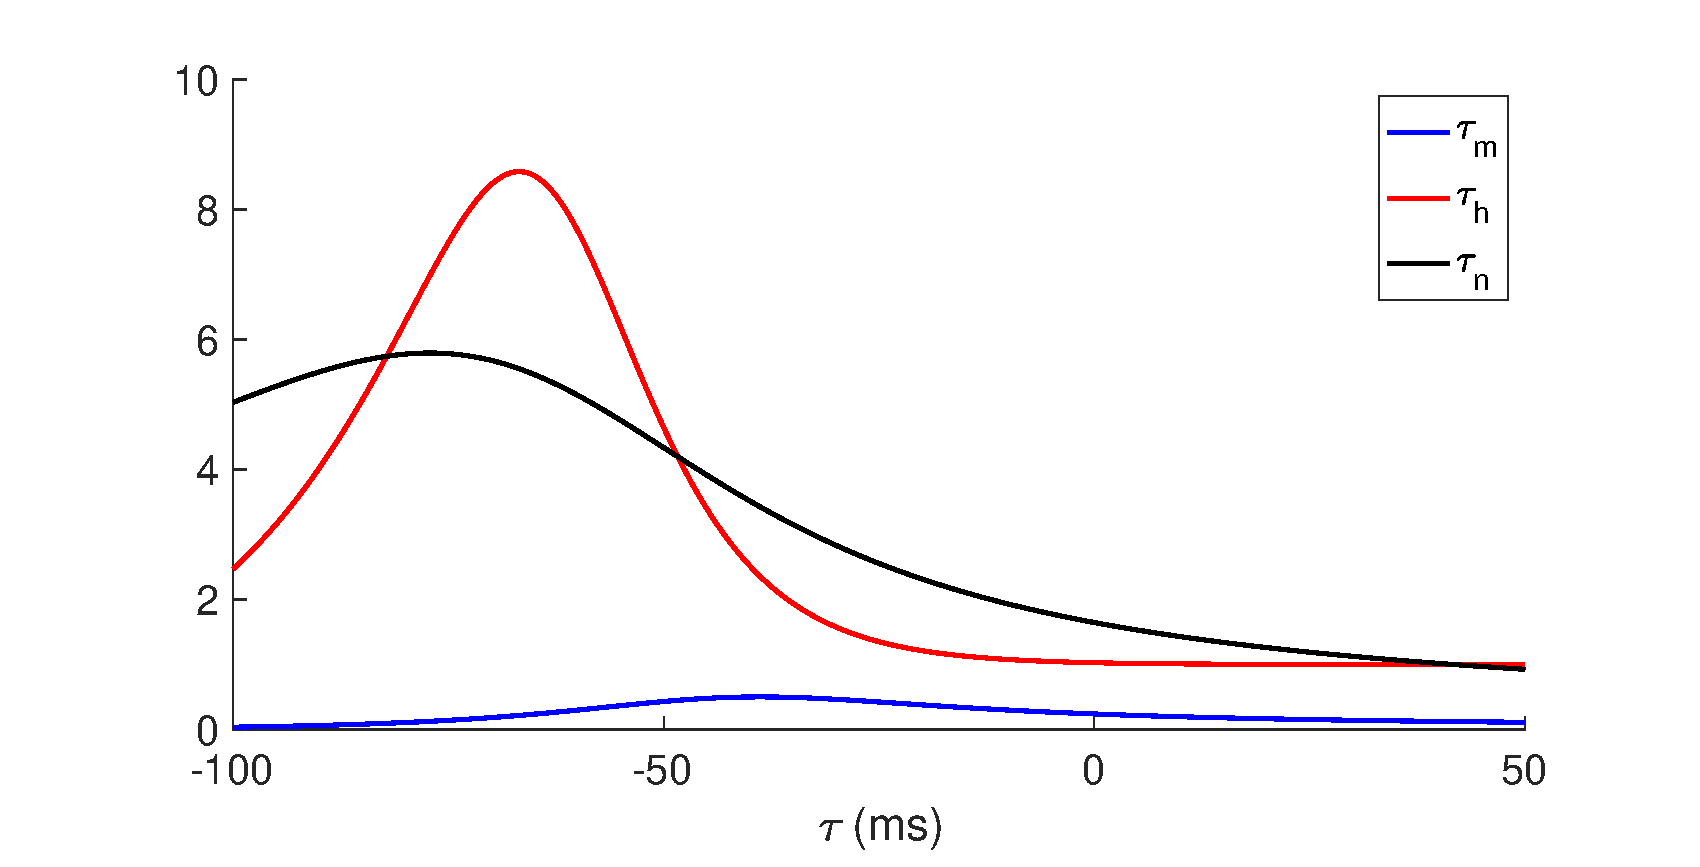
\includegraphics[width=1\linewidth]{Images/photo1_2.eps}
\end{center}
  \end{minipage} 
  \caption{\textbf{Steady state activation/inactivation curves and time constants in the Hodgkin-Huxley model.} Left: steady state activation/inactivation curves. Right: activation/inactivation time constants.}
  \label{photo1}
\end{figure}

\subsection{Conductance-Based models}
The original Hodgkin-Huxley model previously presented, was developed using data from the giant axon of the squid and conductance $Na^{+}$ and $K^{+}$ dynamics were experimentally determined for this case.

However, the same formalism can be used to study most neurons with different conductance dynamics. Neuron models based on these ideas are known as conductance-based models. Conductance-based models can reproduce with quite accuracy the complex behaviour of real neurons.

Each conductance is associated with a reversal potential $E$, a maximal conductance $\bar{g}$, integer exponents $p$ and $q$, and gating variables $m$ and $h$. Each ionic current is described as

\begin{equation}
    I_{ion} = \bar{g}m^{p}h^{q}(V-E)
\end{equation}

Gating variables $m$ and $h$ are known respectively as activation and inactivation variables and satisfy a first order differential equation of identical form

\begin{equation}
    \frac{dX}{dt} = \frac{X_{\infty}(V)-X}{\tau_{X}}
\end{equation}

where $X = m,h$ represents a generic gating variable. Functions $X_{\infty}(V)$ and $\tau_{X}$ are determined from experimental data for each specific neuron.

Gating variables represent the opening and closing dynamics of gating channels, and their dynamics can also be expressed in terms of the channel opening ($\alpha_{X}$) and closing rates $(\beta_{X})$

\begin{equation}
    \frac{dX}{dt} = \alpha_{X}(1-X) - \beta_{X}X
\end{equation}

Research on conductance-based models focus on understanding how the properties of membrane and synaptic conductances give rise to different neural responses. When different ionic currents give rise to similar activity, degeneracy emerge. Thus, conductace-based models have been widely used in the study of the degeneracy problem.

\subsubsection{An example of a conductance-based model}
As an example of a single-compartment, conductance-based biophysical model, we present the model for cells in the internal segment of the globus pallidus (GPi), \cite{Rubin2004,Terman2002} which is used  in the \textit{STN-GPe-GPi-TC} network for GPi cells.

The model includes spiking producing currents sodium ($I_{Na}$) and potassium ($I_{K}$) currents and a leak current ($I_{L}$). Each cell contains also the following types of ionic currents: a calcium activated, voltage-independent afterhyperpolarization potassium current ($I_{AHP}$), a high threshold calcium current ($I_{Ca}$) and a low threshold T-type calcium current ($I_{T}$). These additional ionic currents, based on experimental data, allows the model to reflect $\textit{in vivo}$ firing patterns and they are responsible of most firing properties displayed by GPi cells.

In addition GPi cells receives synaptic current ($I_{syn}$) and applied current ($I_{app}$). For the moment we neglect the synaptic current ($I_{syn}$) ans focus on the single cell model. Overall, each GPi cell is described by a set of five differential equation of the form

\begin{equation}
    C\frac{dV}{dt} = -I_{L} - I_{K} - I_{Na} - I_{T} - I_{Ca} - I_{AHP} + I_{app}
\end{equation}

\begin{equation}
    \frac{dX}{dt} = \Phi_{X} \left( \frac{X_{\infty}(V)-X}{\tau_{X}(V)} \right), \hspace{0.5cm} X=n,h \text{ and } r
\end{equation}
\begin{equation}
    \frac{d[Ca]}{dt} = \varepsilon(-I_{L}-I_{T}-K_{Ca}[Ca])
    \label{ref1}
\end{equation}

The leak current and voltage-dependent currents are given by the Hodgkin-Huxley formalism by

\begin{equation}
    I_{L} = \bar{g}_{L}(V-E_{L})
\end{equation}
\begin{equation}
    I_{K} = \bar{g}_{k}n^{4}(V-E_{K})
\end{equation}
\begin{equation}
    I_{Na} = \bar{g}_{k}m_{\infty}^{3}(V)h(V-E_{Na})
\end{equation}
\begin{equation}
    I_{T} = \bar{g}_{T}a_{\infty}(V)r(V-E_{T})
\end{equation}
\begin{equation}
    I_{Ca} = \bar{g}_{Ca}s_{\infty}^{2}(V)(V-E_{Ca})
\end{equation}

In addition the model presents a calcium-dependent current, the afterhyperpolarization potassium current (AHP) of the form

\begin{equation}
    I_{AHP} = \bar{g}_{AHP}(V-E_{AHP})\left(\frac{[Ca]}{[Ca]+k_{1}} \right)
\end{equation}

where the intracellular concentration of calcium ions ($Ca^{2+}$) is given by Eq. (\ref{ref1}).

Fig. (\ref{photo2}) shows voltage traces for GPi neurons for different levels of applied currents. GPi can fire rapid periodic spikes with sufficient applied current. They also display bursts of activity when subjected to small constant hyperpolarization current.

\begin{figure}[h]
  \begin{minipage}{0.5\linewidth}
  \begin{center}
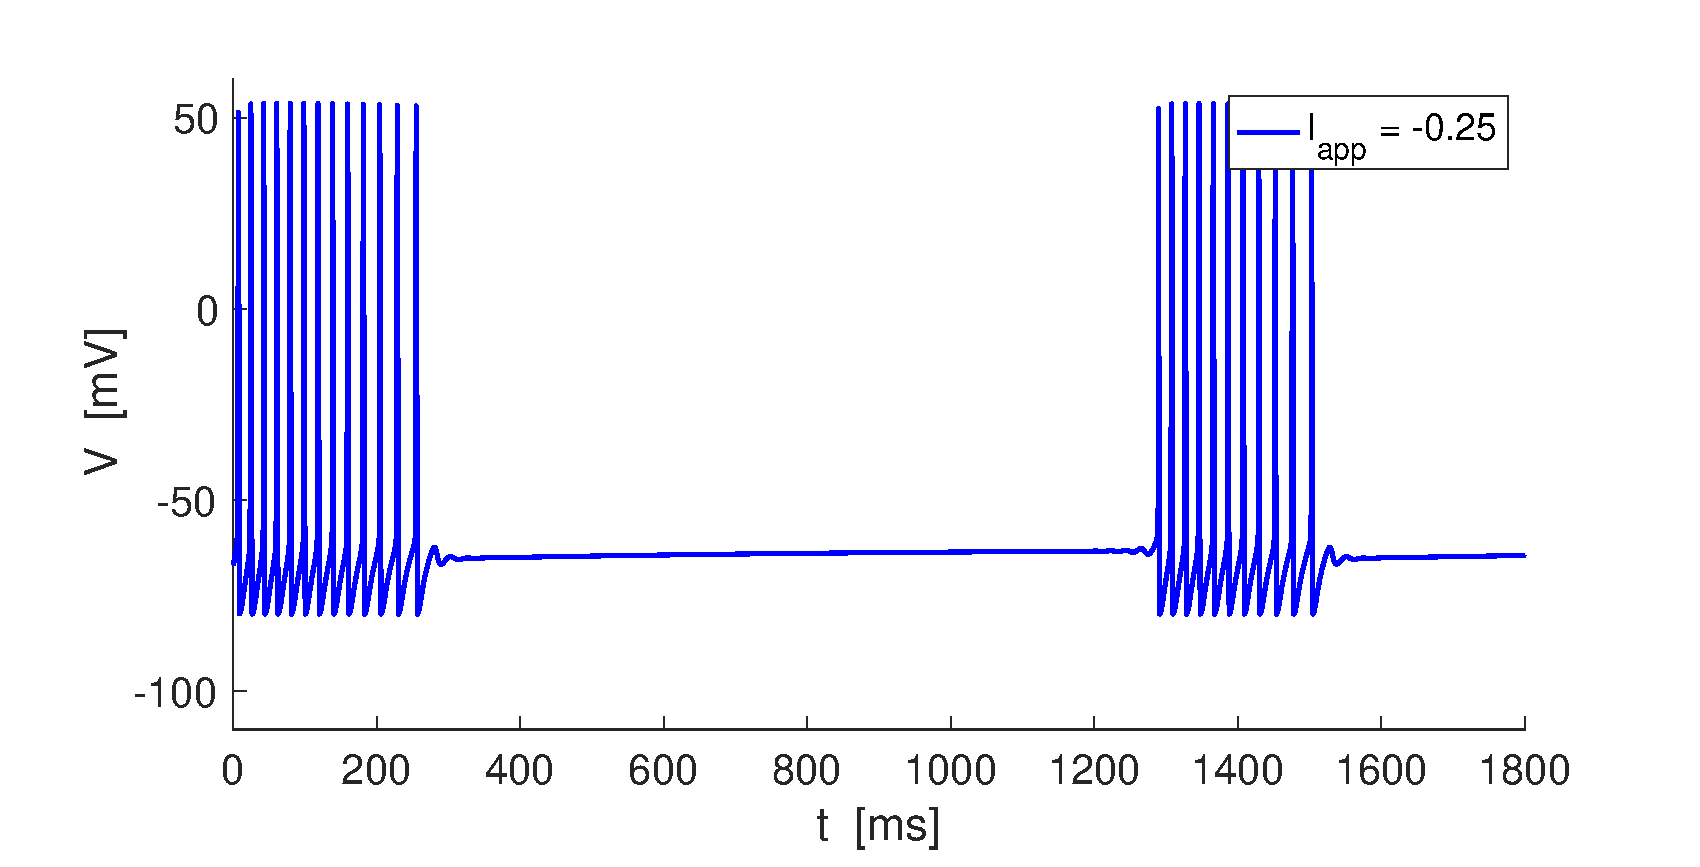
\includegraphics[width=1\linewidth]{Images/photo2_1.eps}
\end{center}
  \end{minipage} 
  \begin{minipage}{0.5\linewidth}
  \begin{center}
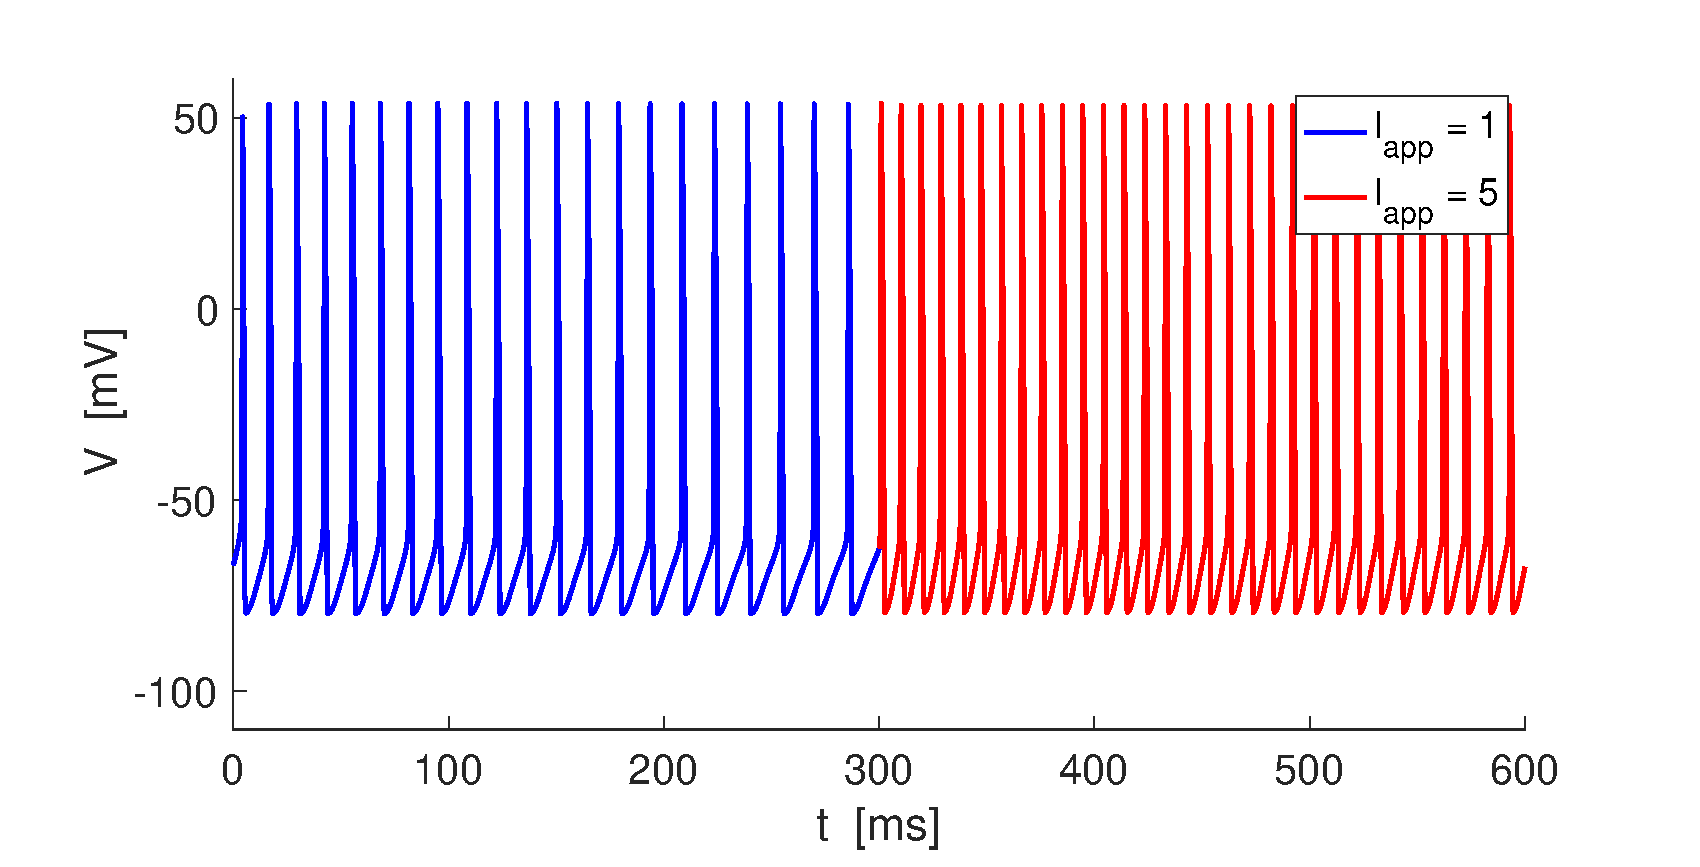
\includegraphics[width=1\linewidth]{Images/photo2_2.eps}
\end{center}
  \end{minipage} 
  \caption{\textbf{Voltage traces for GPi cells for different levels of applied current} Left: GPi cells fire burst of spikes for small negative applied current. Right: GPi cells fire rapid periodic spikes under positive input.}
  \label{photo2}
\end{figure}


\subsection{Reduced models}
Most conductance-based models involve a large number of dynamic variables which make it difficult to carry out a mathematical analysis. Reduced models, in which the number of dynamic variables has been reduced, are of mathematical interest since powerful dynamical system tools such as phase-plane analysis can be performed.

There exist several techniques that can be used to reduce high-dimensional neuron models. For instance, when the voltage-dependent time constant for a particular gating variable ($\tau_{X}$) is much smaller than the rest, the gating variable can be replaced by its stationary solution ($X_{\infty}$) and the dimensionality of the model is reduced by one.

Despite of the importance of these techniques, we will merely present a couple of two-variable models, which have been widely used across computational neuroscience community. Moreover both models presented here, have been used in the study of the degeneracy problem, \cite{Rot,Iii2019}, what make them relevant to our work.

\subsubsection{The Morris-Lecar model}
One of them is the well-known Morris and Lecar model (ML model). Although its simplicity, it is able to exhibit many of the properties displayed by neurons.

The ML model has three channels: a potassium channel, a leak and a calcium channel and it is assumed that the calcium current depends instantaneously on the voltage. The ML equations have the form

\begin{equation}
    C\frac{dV}{dt} = - \bar{g}_{L}(V-E_{L}) - \bar{g}_{K}n(V-E_{K}) - \bar{g}_{Ca}m_{\infty}(V)(V-E_{Ca})
\end{equation}
\begin{equation}
    \frac{dn}{dt} = \frac{n_{\infty}-n}{\tau_{n}(V)}
\end{equation}

where

\begin{equation}
    m_{\infty}(V) = \frac{1}{2}\left(1+tanh((V-V_{2})/V_{2}) \right)
\end{equation}
\begin{equation}
    \tau_{n}(V) = \frac{1}{cosh((V-V_{3})/(2V_{4}))}
\end{equation}
\begin{equation}
 n_{\infty}(V) = \frac{1}{2}\left(1+tanh((V-V_{3})/V_{4}) \right)
\end{equation}

Here, parameters $V_{1}$, $V_{2}$,$V_{3}$ and $V_{4}$ are parameters chosen to fit experimental data.

\subsubsection{The Fitzhugh-Nagumo model}
The second model is the Fitzhugh-Nagumo model (FHN model), \cite{Rot}. In fact, we present here a slightly different version from the original FHN model, \cite{4066548,Fitzhugh1960}. The model is given by 

\begin{equation}
    \frac{dV}{dt} = -hV^{3} + aV^{2} - w
\end{equation}
\begin{equation}
    \frac{dw}{dt} = \varepsilon(\alpha v-\lambda-w)
\end{equation}

where variables $V$ and $w$ describe the voltage and the gating variable, respectively. Furthermore,  parameters $h,a,\alpha, \varepsilon >0$ while parameter $\lambda$ can be any real number.

As well as the ML model, the FHN captures many of the properties of more complex biophysical models. In contrast, unlike the ML model, the FHN model is a simplified neuron model which do not have a biophysical derivation, but shares most mathematical properties with biophysical neuron models.

\section{Synaptic dynamics models}
In building a neuron cell network, it is necessary to determine how neurons are coupled to each other. The main difference between electrical and chemical synapses is that electrical synapses involve a continuous communications between neurons, in contrast with chemical synapses, when the communication is produced when an action potential reach the presynaptic neuron.

\subsection{Electrical synapses}
When cells communicate each other via tight junctions between their membranes, they are synaptically connected via electrical or gap junctions. The synaptic current of the postsynaptic neuron due to an electrical synapse is given by
\begin{equation}
    I_{e} = \bar{g}_{e}(V_{pre}-V_{post})
\end{equation}
where $V_{pre}$ and $V_{post}$ are the corresponding voltages of presynaptic and postsynaptic neurons respectively.

\subsection{Chemical synapses}
At a chemical synapses, presynaptic firing results in the release of transmitter. Binding to receptors on the postsynaptic neuron leads to the opening of ion channels which induces a change in the membrane conductance of the postsynaptic neuron at the site of the synapse. Traditionally, synapses are classified as excitatory or inhibitory, depending on whether they tend to depolarize or hyperpolarize a neuron (enhance firing or not).

The synaptic current for the postsynaptic neuron can be written 

\begin{equation}
    I_{s} = \bar{g}_{s}s(E_{s}-V_{post})
\end{equation}

where $E_{s}$ is the synaptic reversal potential and $\bar{g}_{s}$ the maximal synaptic conductance. The synaptic variable $s$ is related with both the probability that transmitter is released by the presynpatic neuron when it receives the arrival of an action potential and the probability that a postsynaptic channel opens, given that the transmitter was released by the presynaptic neuron.

In a simple synaptic model, it is assumed a transmitter release when an action potential reach the presynaptic neuron. Then, the change with time of the probability that a postsynaptic channel opens can be expressed as

\begin{equation}
    \frac{ds}{dt} = \alpha_{s}(1-s)-\beta_{s}s
\end{equation}

where $\beta_{s}$ determines the closing rate of the channel and is usually assumed to be constant. The opening rate, $\alpha_{s}$, however, has a higher dependence on transmitter concentration. When an action potential reaches the presynaptic neuron, the transmitter concentration rises and $\alpha_{s}$ increases rapidly, causing $s$ to increase. Following the release of transmitter there is a rapid reduction of the transmitter concentration.

\subsubsection{An example of a chemical synapse}
Considering the \textit{STN-GPe-GPi-TC} network model and, as an example of a chemical synapses, we summarize how synaptic currents were modeled in this realistic network.

For instance, synaptic current from a GPe cell (e) to a GPi cell (i) is given by

\begin{equation}
    I_{e\rightarrow i} = \bar{g}_{e\rightarrow i}s_{e}(V_{e}-E_{e\rightarrow i})
\end{equation}

The synaptic variable $s_{e}$ satisfies a first order differential equation of the form

\begin{equation}
    \frac{ds_{e}}{dt} = \alpha_{e}(1-s_{e})H_{\infty}(V_{e}-\theta_{T}) - \beta_{e}s_{e}
    \label{ref2}
\end{equation}

where $H_{\infty}$ is a smooth approximation of the Heaviside function. Here, $\alpha_{e}$ and $\beta_{e}$ represent the rates at which the synapse turn on and turn off and $\theta_{T}$ is a voltage threshold for the presynaptic voltage neuron. Tab. (\ref{t1}) shows the synaptic parameter values.

\begin{table}[h]
	\begin{tabularx}{\textwidth}{X | X | X}
		%\hline
		$\alpha_{e}$		& $\beta_{e}$			& $\theta_{T}$  \\ \hline
		1			& 0.1			& -20				\\ 
	\end{tabularx}
	\caption{Synaptic parameter values.}
	\label{t1}
\end{table}

Figure (\ref{photo3}) shows the synaptic conductance as a function of time due a single presynaptic spike on a GPe cell. We note that synaptic variable $s_{e}$ increases when presynaptic GPe voltage is higher than the voltage threshold $\theta_{e}$. It starts to decrease when the action potential terminates and voltage is lower than the voltage threshold $\theta_{T}$.

\begin{figure}[h]
  \begin{minipage}{0.5\linewidth}
  \begin{center}
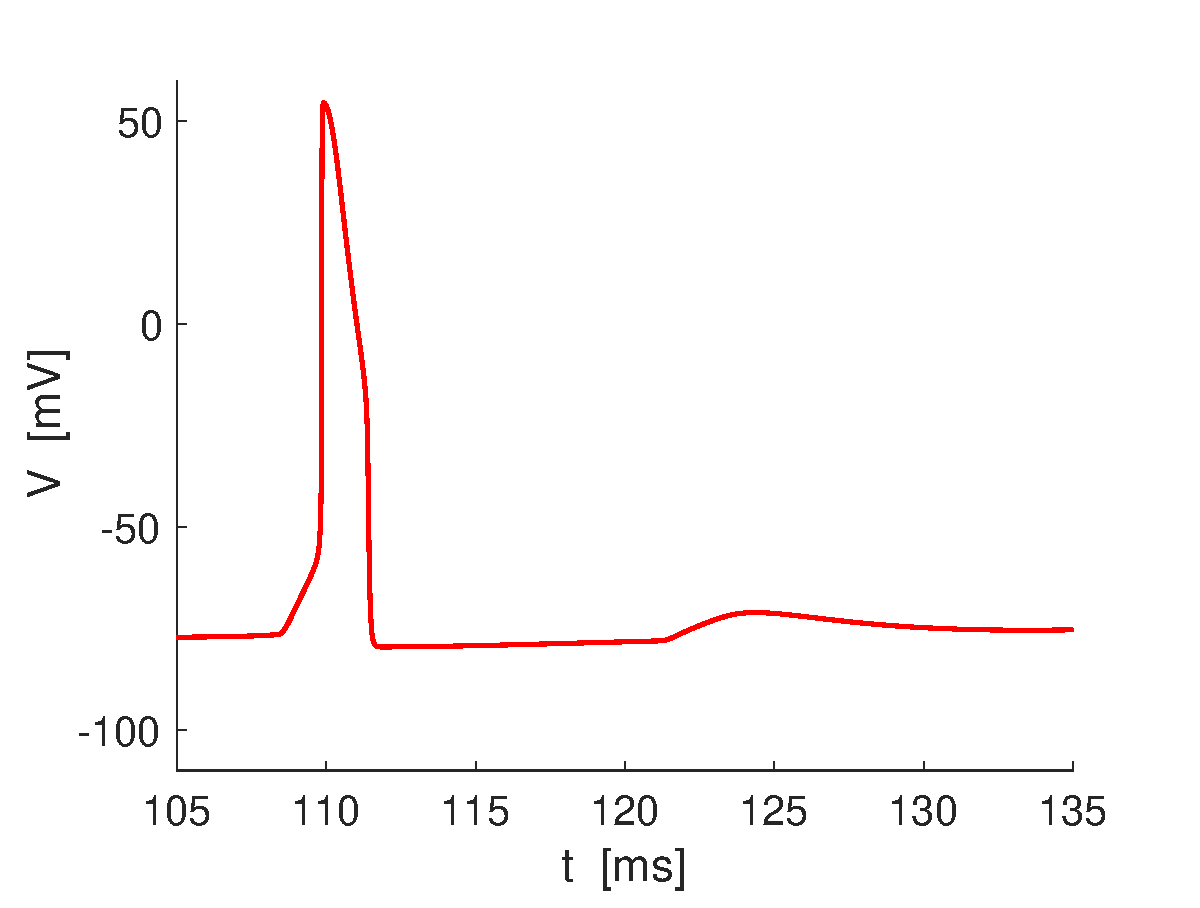
\includegraphics[width=1\linewidth]{Images/photo3_1.eps}
\end{center}
  \end{minipage} 
  \begin{minipage}{0.5\linewidth}
  \begin{center}
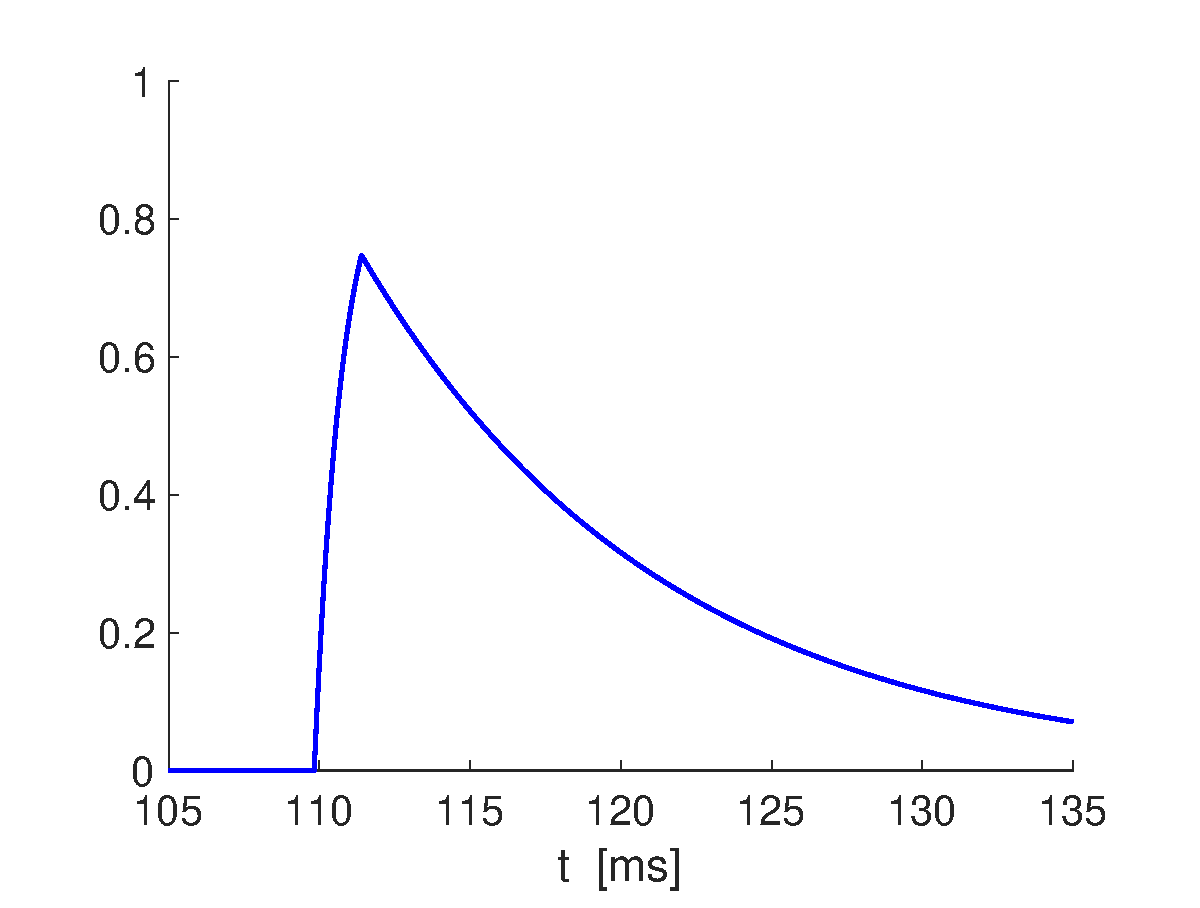
\includegraphics[width=1\linewidth]{Images/photo3_2.eps}
\end{center}
  \end{minipage} 
  \caption{\textbf{Synaptic conductance model in the \textit{STN-GPe-GPi-TC} network.} Left: single presynaptic spike on a GPe cell. Right: conductance due to a single spike on presynaptic GPe cell (left).}
  \label{photo3}
\end{figure}



\section{Mathematical Models for Neuronal Networks}
One described single cell models and synaptic models, we describe some mathematical models for neuron networks.

Apparently, the most direct way to simulate neural network is to synaptically connect model spiking neurons, such as conductance based models. This is how mathematical models for neuronal networks are built in this section. However, we notice the existence of other neural network models, such as Firing-Rate models, which are widely used in computational neuroscience. Firing-Rate models, instead of voltage, use as an output the firing rate, which is a measure of the number of spikes generated per unit of time.

Despite the importance of Firing-Rate models in computational neuroscience, we focus on neuronal network built connecting single neuron spiking models, since mathematical networks considered in this work are inspired by these type of neural networks.

We note that network properties depends on individual cells, synaptic connections between cells and the network architecture. Networks architectures, such as random or structured are possible in networks involving a large number of neurons.

In order to illustrate neural network models, we build two-neuron electrically and chemically fully connected networks. Without loss of generality, we consider a general two-variable neuron model to describe the behaviour of each neuron in the network with general form

\begin{equation}
    \frac{dV}{dt}  = f(V,w)
\end{equation}
\begin{equation}
    \frac{dw}{dt}  = g(V,w)
\end{equation}

where $V$ is the membrane potential of the cell and $w$ a channel gating variable.

\subsection{Electrical networks}
The model for a pair of mutually electrically coupled neurons is given by

\begin{equation}
    \frac{dV_{i}}{dt}  = f_{i}(V_{i},w_{i}) - \bar{g}_{j}^{i}(V_{i}-V_{j})
\end{equation}
\begin{equation}
    \frac{dw_{i}}{dt}  = g_{i}(V_{i},w_{i})
\end{equation}

where $i,j = 1 $ or $2$ and $i \neq j$ and $\bar{g}_{j}^{i}$ is the maximal conductance for synaptic current from neuron $i$ to neuron $j$.


\subsection{Chemical networks}
For chemical synapses, we assume synaptic variable $s$ satisfies a first-order differential equation of the form in Eq. (\ref{ref2}), previously studied.

The model for a pair of mutually chemically coupled neurons is then

\begin{equation}
    \frac{dV_{i}}{dt}  = f_{i}(V_{i},w_{i}) - \bar{g}_{s}^{i}s_{j}(V_{i}-E_{s}^{i})
\end{equation}
\begin{equation}
    \frac{dw_{i}}{dt}  = g_{i}(V_{i},w_{i})
\end{equation}
\begin{equation}
    \frac{ds_{i}}{dt}  = \alpha_{s}^{i}(1-s_{i})H_{\infty}(V_{i}-\theta_{T}^{i})-\beta_{s}^{i}s_{i}
\end{equation}

where $i,j = 1 $, $2$ and $i \neq j$.

Network models presented, correspond to the most general heterogeneous network, in which cells have different intrinsic parameters.
